Now that we have identified the basic building blocks for efficient communication between work-items, we can describe how to express work-group barriers and local memory in kernels. Remember that communication between work-items requires a notion of work-item grouping, so these concepts can only be expressed for ND-range kernels and hierarchical kernels and are not included in the execution model for basic data-parallel kernels.\par

This chapter will build upon the naïve matrix multiplication kernel examples introduced in Chapter 4 by introducing communication between the work-items in the work-groups executing the matrix multiplication. On many devices—but not necessarily all!—communicating through local memory will improve the performance of the matrix multiplication kernel.\par

\begin{tcolorbox}[colback=blue!5!white,colframe=blue!75!black, title=A NOTE ABOUT MATRIX MULTIPLICATION]
In this book, matrix multiplication kernels are used to demonstrate how changes in a kernel affect performance. Although matrix multiplication performance may be improved on some devices using the techniques described in this chapter, matrix multiplication is such an important and common operation that many vendors have implemented highly tuned versions of matrix multiplication. Vendors invest significant time and effort implementing and validating functions for specific devices and in some cases may use functionality or techniques that are difficult or impossible to use in standard parallel kernels.
\end{tcolorbox}

\begin{tcolorbox}[colback=blue!5!white,colframe=blue!75!black, title=USE VENDOR-PROVIDED LIBRARIES!]
When a vendor provides a library implementation of a function, it is almost always beneficial to use it rather than re-implementing the function as a parallel kernel! For matrix multiplication, one can look to oneMKL as part of Intel’s oneAPI toolkits for solutions appropriate for DPC++ programmers.
\end{tcolorbox}

Figure 9-4 shows the naïve matrix multiplication kernel we will be starting from, taken from Chapter 4.\par

\hspace*{\fill} \par %插入空行
Figure 9-4. The naïve matrix multiplication kernel from Chapter 4
\begin{lstlisting}[caption={}]
h.parallel_for(range{M, N}, [=](id<2> id) {
	int m = id[0];
	int n = id[1];
	
	T sum = 0;
	for (int k = 0; k < K; k++)
		sum += matrixA[m][k] * matrixB[k][n];
		
	matrixC[m][n] = sum;
});
\end{lstlisting}

In Chapter 4, we observed that the matrix multiplication algorithm has a high degree of reuse and that grouping work-items may improve locality of access which may improve cache hit rates. In this chapter, instead of relying on implicit cache behavior to improve performance, our modified matrix multiplication kernels will instead use local memory as an explicit cache, to guarantee locality of access.\par

\begin{tcolorbox}[colback=red!5!white,colframe=red!75!black]
For many algorithms, it is helpful to think of local memory as an explicit cache.
\end{tcolorbox}

Figure 9-5 is a modified diagram from Chapter 4 showing a work-group consisting of a single row, which makes the algorithm using local memory easier to understand. Observe that for elements in a row of the result matrix, every result element is computed using a unique column of data from one of the input matrices, shown in blue and orange. Because there is no data sharing for this input matrix, it is not an ideal candidate for local memory. Observe, though, that every result element in the row accesses the exact same data in the other input matrix, shown in green. Because this data is reused, it is an excellent candidate to benefit from work-group local memory.\par

\hspace*{\fill} \par %插入空行
Figure 9-5. Mapping of matrix multiplication to work-groups and work-items
\begin{center}
	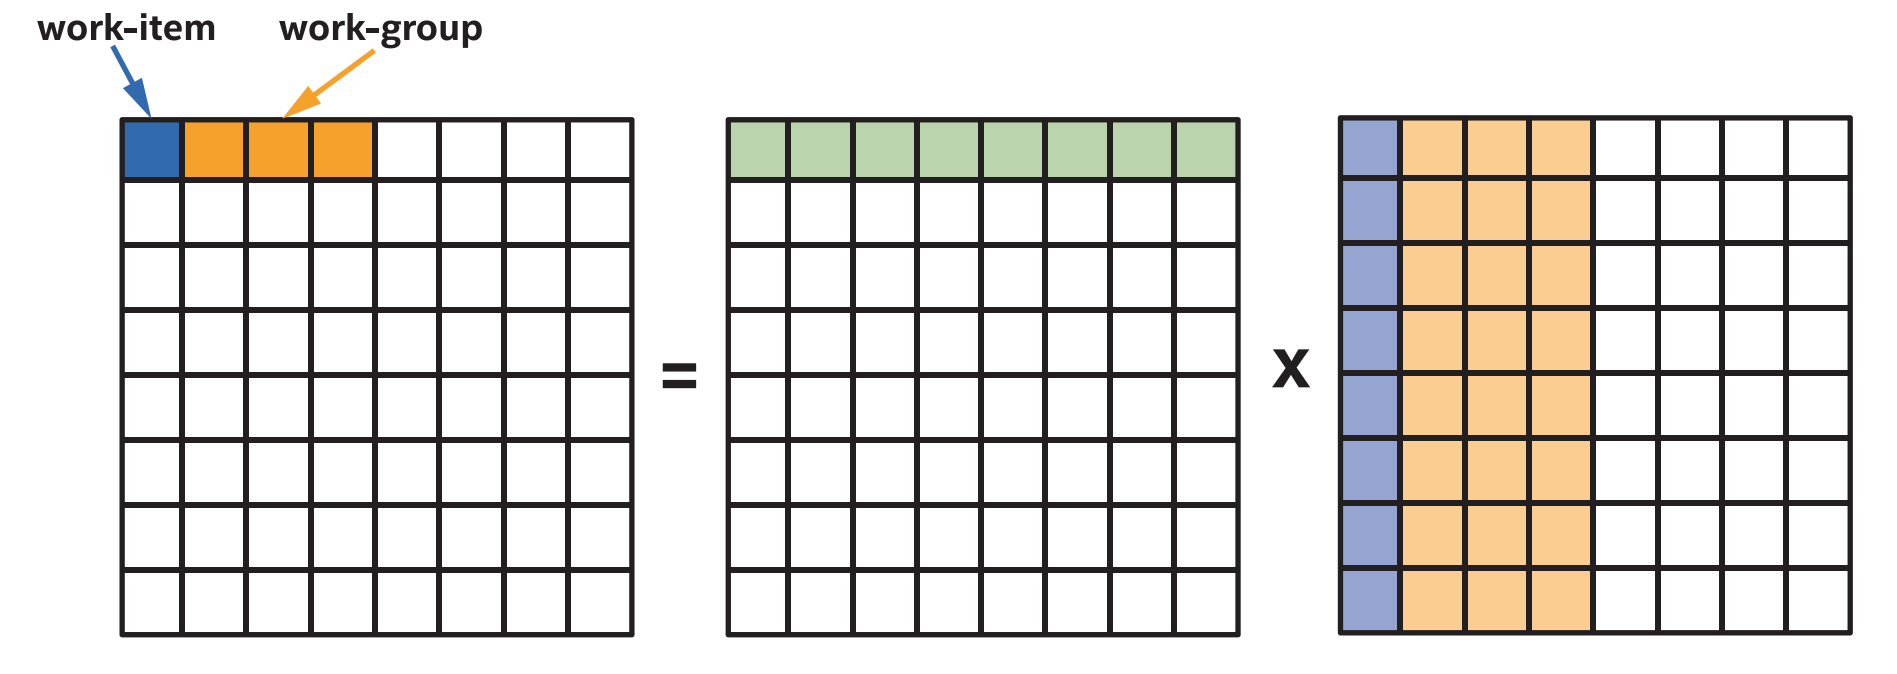
\includegraphics[width=1.\textwidth]{content/chapter-9/images/5}
\end{center}

Because we want to multiply matrices that are potentially very large and because work-group local memory may be a limited resource, our modified kernels will process subsections of each matrix, which we will refer to as a matrix tile. For each tile, our modified kernel will load data for the tile into local memory, synchronize the work-items in the group, and then load the data from local memory rather than global memory. The data that is accessed for the first tile is shown in Figure 9-6.\par

In our kernels, we have chosen the tile size to be equivalent to the work-group size. This is not required, but because it simplifies transfers into or out of local memory, it is common and convenient to choose a tile size that is a multiple of the work-group size.\par

\hspace*{\fill} \par %插入空行
Figure 9-6. Processing the first tile: the green input data (left of X) is reused and is read from local memory, the blue and orange input data (right of X) is read from global memory
\begin{center}
	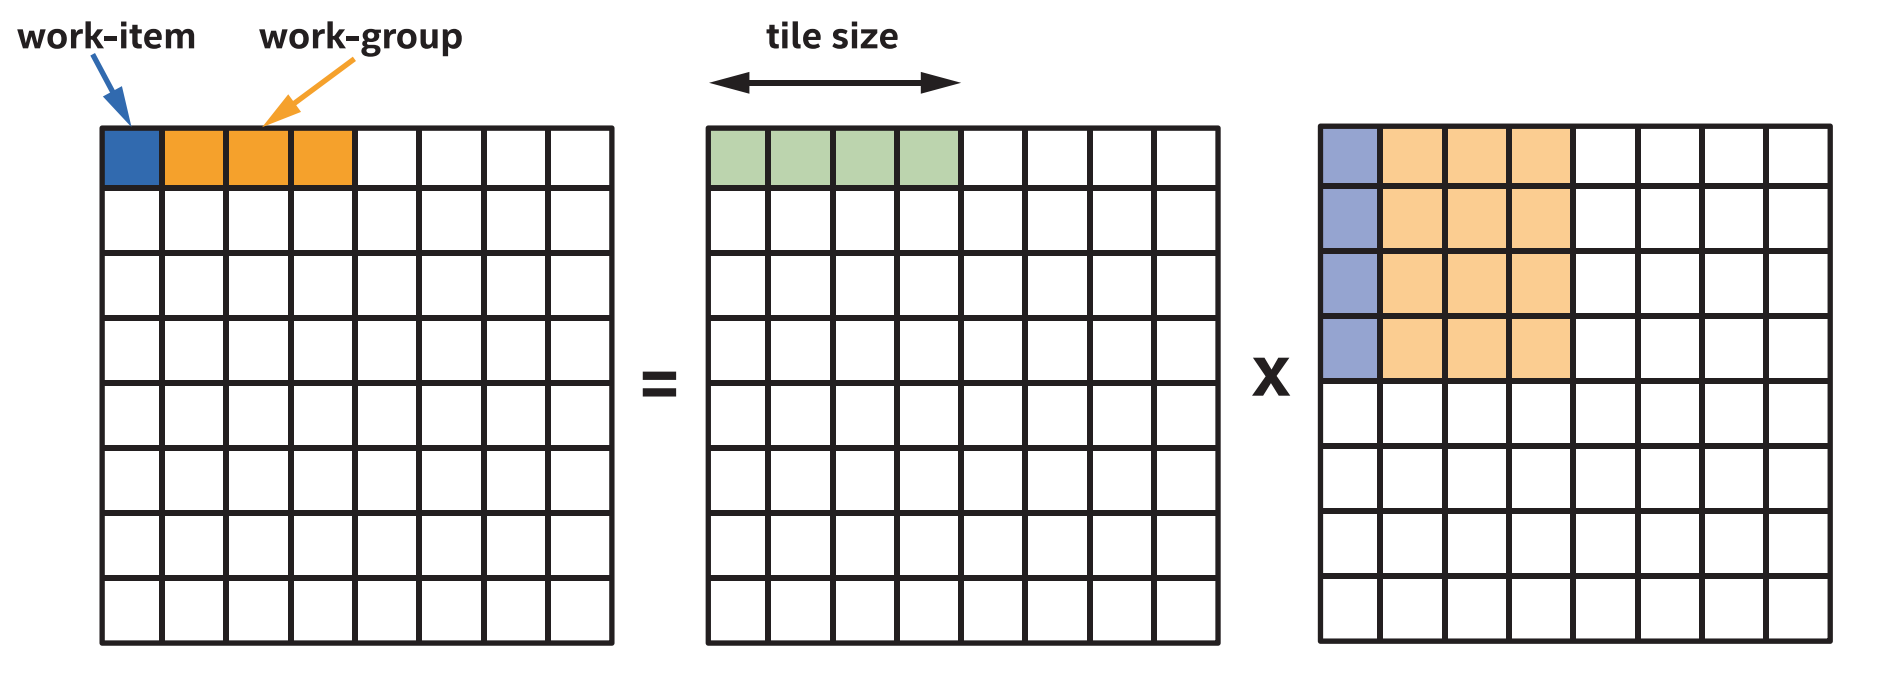
\includegraphics[width=1.\textwidth]{content/chapter-9/images/6}
\end{center}

\hspace*{\fill} \par %插入空行
\textbf{Work-Group Barriers and Local Memory in ND-Range Kernels}

This section describes how work-group barriers and local memory are expressed in ND-range kernels. For ND-range kernels, the representation is explicit: a kernel declares and operates on a local accessor representing an allocation in the local address space and calls a barrier function to synchronize the work-items in a work-group.\par

\hspace*{\fill} \par %插入空行
\textbf{Local Accessors}

To declare local memory for use in an ND-range kernel, use a local accessor. Like other accessor objects, a local accessor is constructed within a command group handler, but unlike the accessor objects discussed in Chapters 3 and 7, a local accessor is not created from a buffer object. Instead, a local accessor is created by specifying a type and a range describing the number of elements of that type. Like other accessors, local accessors may be one-dimensional, two-dimensional, or threedimensional. Figure 9-7 demonstrates how to declare local accessors and use them in a kernel.\par

Remember that local memory is uninitialized when each work-group begins and does not persist after each work-group completes. This means that a local accessor must always be read\_write, since otherwise a kernel would have no way to assign the contents of local memory or view the results of an assignment. Local accessors may optionally be atomic though, in which case accesses to local memory via the accessor are performed atomically. Atomic accesses are discussed in more detail in Chapter 19.\par

\hspace*{\fill} \par %插入空行
Figure 9-7. Declaring and using local accessors
\begin{lstlisting}[caption={}]
// This is a typical global accessor.
accessor dataAcc {dataBuf, h};

// This is a 1D local accessor consisting of 16 ints:
local_accessor<int> localIntAcc{16, h};

// This is a 2D local accessor consisting of 4 x 4 floats:
local_accessor<float,2> localFloatAcc{{4,4}, h};

h.parallel_for(nd_range<1>{{size}, {16}}, [=](nd_item<1> item) {
	auto index = item.get_global_id();
	auto local_index = item.get_local_id();
	
	// Within a kernel, a local accessor may be read from
	// and written to like any other accessor.
	localIntAcc[local_index] = dataAcc[index] + 1;
	dataAcc[index] = localIntAcc[local_index];
});
\end{lstlisting}

\hspace*{\fill} \par %插入空行
\textbf{Synchronization Functions}

To synchronize the work-items in an ND-range kernel work-group, call the barrier function in the nd\_item class. Because the barrier function is a member of the nd\_item class, it is only available to ND-range kernels and is not available to basic data-parallel kernels or hierarchical kernels.\par

The barrier function currently accepts one argument to describe the memory spaces to synchronize or fence, but the arguments to the barrier function may change in the future as the memory model evolves in SYCL and DPC++. In all cases though, the arguments to the barrier function provide additional control regarding the memory spaces that are synchronized or the scope of the memory synchronization.\par

When no arguments are passed to the barrier function, the barrier function will use functionally correct and conservative defaults. The code examples in this chapter use this syntax for maximum portability and readability. For highly optimized kernels, it is recommended to precisely describe which memory spaces or which work-items must be synchronized, which may improve performance.\par

\hspace*{\fill} \par %插入空行
\textbf{A Full ND-Range Kernel Example}

Now that we know how to declare a local memory accessor and synchronize access to it using a barrier function, we can implement an ND-range kernel version of matrix multiplication that coordinates communication among work-items in the work-group to reduce traffic to global memory. The complete example is shown in Figure 9-8.\par

\hspace*{\fill} \par %插入空行
Figure 9-8. Expressing a tiled matrix multiplication kernel with an ND-range parallel\_for and work-group local memory
\begin{lstlisting}[caption={}]
// Traditional accessors, representing matrices in global memory:
accessor matrixA{bufA, h};
accessor matrixB{bufB, h};
accessor matrixC{bufC, h};

// Local accessor, for one matrix tile:
constexpr int tile_size = 16;
local_accessor<int> tileA{tile_size, h};

h.parallel_for(
nd_range<2>{{M, N}, {1, tile_size}}, [=](nd_item<2> item) {
	// Indices in the global index space:
	int m = item.get_global_id()[0];
	int n = item.get_global_id()[1];
	
	// Index in the local index space:
	int i = item.get_local_id()[1];
	
	T sum = 0;
	for (int kk = 0; kk < K; kk += tile_size) {
		// Load the matrix tile from matrix A, and synchronize
		// to ensure all work-items have a consistent view
		// of the matrix tile in local memory.
		tileA[i] = matrixA[m][kk + i];
		item.barrier();
		
		// Perform computation using the local memory tile, and
		// matrix B in global memory.
		for (int k = 0; k < tile_size; k++)
			sum += tileA[k] * matrixB[kk + k][n];
		
		// After computation, synchronize again, to ensure all
		// reads from the local memory tile are complete.
		item.barrier();
	}

	// Write the final result to global memory.
	matrixC[m][n] = sum;
});
\end{lstlisting}

The main loop in this kernel can be thought of as two distinct phases: in the first phase, the work-items in the work-group collaborate to load shared data from the A matrix into work-group local memory; and in the second, the work-items perform their own computations using the shared data. In order to ensure that all work-items have completed the first phase before moving onto the second phase, the two phases are separated by a call to barrier to synchronize all work-items and to provide a memory fence. This pattern is a common one, and the use of work-group local memory in a kernel almost always necessitates the use of work-group barriers.\par

Note that there must also be a call to barrier to synchronize execution between the computation phase for the current tile and the loading phase for the next matrix tile. Without this synchronization operation, part of the current matrix tile may be overwritten by one work-item in the work-group before another work-item is finished computing with it. In general, any time that one work-item is reading or writing data in local memory that was read or written by another work-item, synchronization is required. In Figure 9-8, the synchronization is done at the end of the loop, but it would be equally correct to synchronize at the beginning of each loop iteration instead.\par

\hspace*{\fill} \par %插入空行
\textbf{Work-Group Barriers and Local Memory in Hierarchical Kernels}

This section describes how work-group barriers and local memory are expressed in hierarchical kernels. Unlike ND-range kernels, local memory and barriers in hierarchical kernels are implicit, requiring no special syntax or function calls. Some programmers will find the hierarchical kernel representation more intuitive and easier to use, whereas other programmers will appreciate the direct control provided by ND-range kernels. In most cases, the same algorithms may be described using both representations, so we can choose the representation that we find easiest to develop and maintain.\par

\hspace*{\fill} \par %插入空行
\textbf{Scopes for Local Memory and Barriers}

Recall from Chapter 4 that hierarchical kernels express two levels of parallel execution through use of the parallel\_for\_work\_group and parallel\_for\_work\_item functions. These two levels, or scopes, of parallel execution are used to express whether a variable is in work-group local memory and shared across all work-items in the work-group or whether a variable is in per-work-item private memory that is not shared among work-items. The two scopes are also used to synchronize the work-items in a work-group and to enforce memory consistency.\par

Figure 9-9 shows an example hierarchical kernel that declares a variable at work-group scope in local memory, loads into it, and then uses that variable in work-item scope. There is an implicit barrier between the write into local memory at work-group scope and the read from local memory at work-item scope.\par

\hspace*{\fill} \par %插入空行
Figure 9-9. Hierarchical kernel with a local memory variable
\begin{lstlisting}[caption={}]
range group_size{16};
range num_groups = size / group_size;

h.parallel_for_work_group(num_groups, group_size, [=](group<1> group) {
	// This variable is declared at work-group scope, so
	// it is allocated in local memory and accessible to
	// all work-items.
	int localIntArr[16];
	
	// There is an implicit barrier between code and variables
	// declared at work-group scope and the code and variables
	// at work-item scope.
	
	group.parallel_for_work_item([&](h_item<1> item) {
		auto index = item.get_global_id();
		auto local_index = item.get_local_id();
		
		// The code at work-item scope can read and write the
		// variables declared at work-group scope.
		localIntArr[local_index] = index + 1;
		data_acc[index] = localIntArr[local_index];
	});
});
\end{lstlisting}

The main advantage of the hierarchical kernel representation is that it looks very similar to standard C++ code, where some variables may be assigned in one scope and used in a nested scope. Of course, this also may be considered a disadvantage, since it is not immediately obvious which variables are in local memory and when barriers must be inserted by the hierarchical kernel compiler. This is especially true for devices where barriers are expensive!\par

\hspace*{\fill} \par %插入空行
\textbf{A Full Hierarchical Kernel Example}

Now that we know how to express local memory and barriers in hierarchical kernels, we can write a hierarchical kernel that implements the same algorithm as the ND-range kernel in Figure 9-7. This kernel is shown in Figure 9-10.\par

Although the hierarchical kernel is very similar to the ND-range kernel, there is one key difference: in the ND-range kernel, the results of the matrix multiplication are accumulated into the per-work-item variable sum before writing to the output matrix in memory, whereas the hierarchical kernel accumulates into memory. We could accumulate into a per-workitem variable in the hierarchical kernel as well, but this requires a special private\_memory syntax to declare per-work-item data at work-group scope, and one of the reasons we chose to use the hierarchical kernel syntax was to avoid special syntax!\par

\begin{tcolorbox}[colback=red!5!white,colframe=red!75!black]
Hierarchical kernels do not require special syntax to declare variables in work-group local memory, but they require special syntax to declare some variables in work-item private memory!
\end{tcolorbox}

To avoid the special per-work-item data syntax, it is a common pattern for work-item loops in hierarchical kernels to write intermediate results to either work-group local memory or global memory.\par

\hspace*{\fill} \par %插入空行
Figure 9-10. A tiled matrix multiplication kernel implemented as a hierarchical kernel
\begin{lstlisting}[caption={}]
const int tileSize = 16;
range group_size{1, tileSize};
range num_groups{M, N / tileSize};

h.parallel_for_work_group(num_groups, group_size, [=](group<2> group) {
	// Because this array is declared at work-group scope
	// it is in local memory
	T tileA[16];
	
	for (int kk = 0; kk < K; kk += tileSize) {
		// A barrier may be inserted between scopes here
		// automatically, unless the compiler can prove it is
		// not required
		
		// Load the matrix tile from matrix A
		group.parallel_for_work_item([&](h_item<2> item) {
			int m = item.get_global_id()[0];
			int i = item.get_local_id()[1];
			tileA[i] = matrixA[m][kk + i];
		});
	
		// A barrier gets inserted here automatically, so all
		// work items have a consistent view of memory
		
		group.parallel_for_work_item([&](h_item<2> item) {
			int m = item.get_global_id()[0];
			int n = item.get_global_id()[1];
			for (int k = 0; k < tileSize; k++)
			matrixC[m][n] += tileA[k] * matrixB[kk + k][n];
		});
	
		// A barrier gets inserted here automatically, too
	}
});
\end{lstlisting}

One final interesting property of the kernel in Figure 9-10 concerns the loop iteration variable kk: since the loop is at work-group scope, the loop iteration variable kk could be allocated out of work-group local memory, just like the tileA array. In this case though, since the value of kk is the same for all work-items in the work-group, a smart compiler may choose to allocate kk from per-work-item memory instead, especially for devices where work-group local memory is a scarce resource.\par























